\lstset{backgroundcolor = \color{lightgray!20},
  basicstyle=\ttfamily,
  keywordstyle=\color{blue}\ttfamily,
  stringstyle=\color{red}\ttfamily,
  commentstyle=\color[HTML]{31B404}\ttfamily,
  language = Matlab
}

\section{Annotated code}

The Matlab code here is taken from the website: \url{http://cvlab.epfl.ch/software/daisy}.
As said in the code documentation, the code is divided into precomputation and
descriptor computation steps.

\subsection{Compute histograms for each pixel}

The histograms are computed in the precomputation step, ie.\ in the
\textbf{init\_daisy} function.

\begin{lstlisting}
%% compute histograms
h = size(im,1);
w = size(im,2);
for r=1:cn
    dzy.TCL(:,:,:,r) = transpose_cube(dzy.CL(:,:,:,r));
    dzy.H(:,:,r) = reshape( dzy.TCL(:,:,:,r), h*w, HQ );
end
\end{lstlisting}

The variable \textbf{dzy.CL} contains the ``cubes'' of the image. A cube means
the scale-space representation. The variable \textbf{HQ} is the number of bins
in the histogram.
% For reference, here's the \textbf{transpose\_cube} function.
% \begin{lstlisting}
% function tc = transpose_cube( cube )
% [h, w, n]=size(cube);
% tc(w,h,n)=single(0);
% for i=1:n
%     tc(:,:,i) = transpose(cube(:,:,i));
% end
% \end{lstlisting}

\subsection{Normalize histograms to unit norm}

In the code, normalization seems to be done as the last step, after the
descriptor has been computed.
By default, the code uses partial normalization. The argument \textbf{udsc} is
the descriptor.
\begin{lstlisting}
function dsc = normalize_partial(udsc)

gn = size( udsc,1 );
dsc = udsc;
for i=1:gn
    n = norm(udsc(i,:));
    if n~= 0, dsc(i,:) = udsc(i,:)/n; end
end
\end{lstlisting}

For comparison, here is the SIFT-like normalization function.
\begin{lstlisting}
function dsc = normalize_sift(udsc)

threshold = 0.154;
changed = 1;
iter = 0;
max_iter = 5;

dsc = udsc;
while( changed && iter < max_iter )
    iter=iter+1;
    changed = 0;

    dsc=normalize_full(dsc);

    if sum(sum(dsc> threshold)) > 0
        dsc(dsc>threshold) = threshold;
        changed=1;
    end
end
\end{lstlisting}


\subsection{DAISY descriptor is computed}

The matlab code contains 4 DAISY descriptor computing functions, depending on
what interpolation types are enabled. There are two interpolation options
available: \textbf{Spatial interpolation} and \textbf{layered interpolation}.
For brevity's sake this text only contains the function with both interpolation
types enabled.
% The function without any interpolation is:
% \begin{lstlisting}
% function desc = u_compute_descriptor_00(dzy, y, x, orientation)
% HN = dzy.HN;
% HQ = dzy.HQ;

% o = floor(orientation);
% assert( o >= 0 & o< 360 );

% shift  = dzy.ostable(o+1);
% ishift = double(floor(shift));

% desc(HN,HQ)=single(0);


% for h=1:HN
%     ci = dzy.ogrid(h,1,o+1);
%     yy = floor(y + dzy.ogrid(h,2,o+1));
%     xx = floor(x + dzy.ogrid(h,3,o+1));
% %    [yy xx]
%     if (yy < 0) || yy>(dzy.h-1) || (xx<0) || xx>(dzy.w-1)
%         continue;
%     end
%     hist(:,1) = dzy.H( yy*dzy.w+xx+1, :, ci );
%     desc(h,:) = circshift(hist,-ishift);
% end
% \end{lstlisting}

% The function with both types of interpolation enabled is:
\begin{lstlisting}
function desc = u_compute_descriptor_11(dzy, y, x, orientation)

HN = dzy.HN;
HQ = dzy.HQ;

o = floor(orientation);
assert( o >= 0 & o< 360 );

shift  = dzy.ostable(o+1);
ishift = double(floor(shift));

desc(HN,HQ)=single(0);
sdesc(HN,HQ)=single(0);

for h=1:HN
    ci = dzy.ogrid(h,1,o+1);
    yy = y + dzy.ogrid(h,2,o+1);
    xx = x + dzy.ogrid(h,3,o+1);
    iy=floor(yy);
    ix=floor(xx);

    b = yy-iy;
    a = xx-ix;

    if (iy < 0) || iy>(dzy.h-2) || (ix<0) || ix>(dzy.w-2)
        continue;
    end

    % A C
    % B D
    ha(:,1) = dzy.H( iy    *dzy.w+ix+1, :, ci );
    hb(:,1) = dzy.H( (1+iy)*dzy.w+ix+1, :, ci );
    hc(:,1) = dzy.H( iy    *dzy.w+ix+2, :, ci );
    hd(:,1) = dzy.H( (1+iy)*dzy.w+ix+2, :, ci );

    hist = (1-b)*(a*hc+(1-a)*ha)+b*(a*hd+(1-a)*hb);
    sdesc(h,:) = circshift(hist,-ishift);
end

f=shift-ishift;
for i=1:HQ-1
    desc(:,i) = f*sdesc(:,i+1)+(1-f)*sdesc(:,i);
end
desc(:,HQ) = f*sdesc(:,1)+(1-f)*sdesc(:,HQ);
\end{lstlisting}

\section{Directional derivative images}

Figure~\ref{fig:grasshopper} contains one input image and it's 3 directional
derivative images. The amount of directional derivative images is dependant on
(and the same as) the number of layers of DAISY descriptors.


% \begin{figure}[H]\label{fig:face}
%   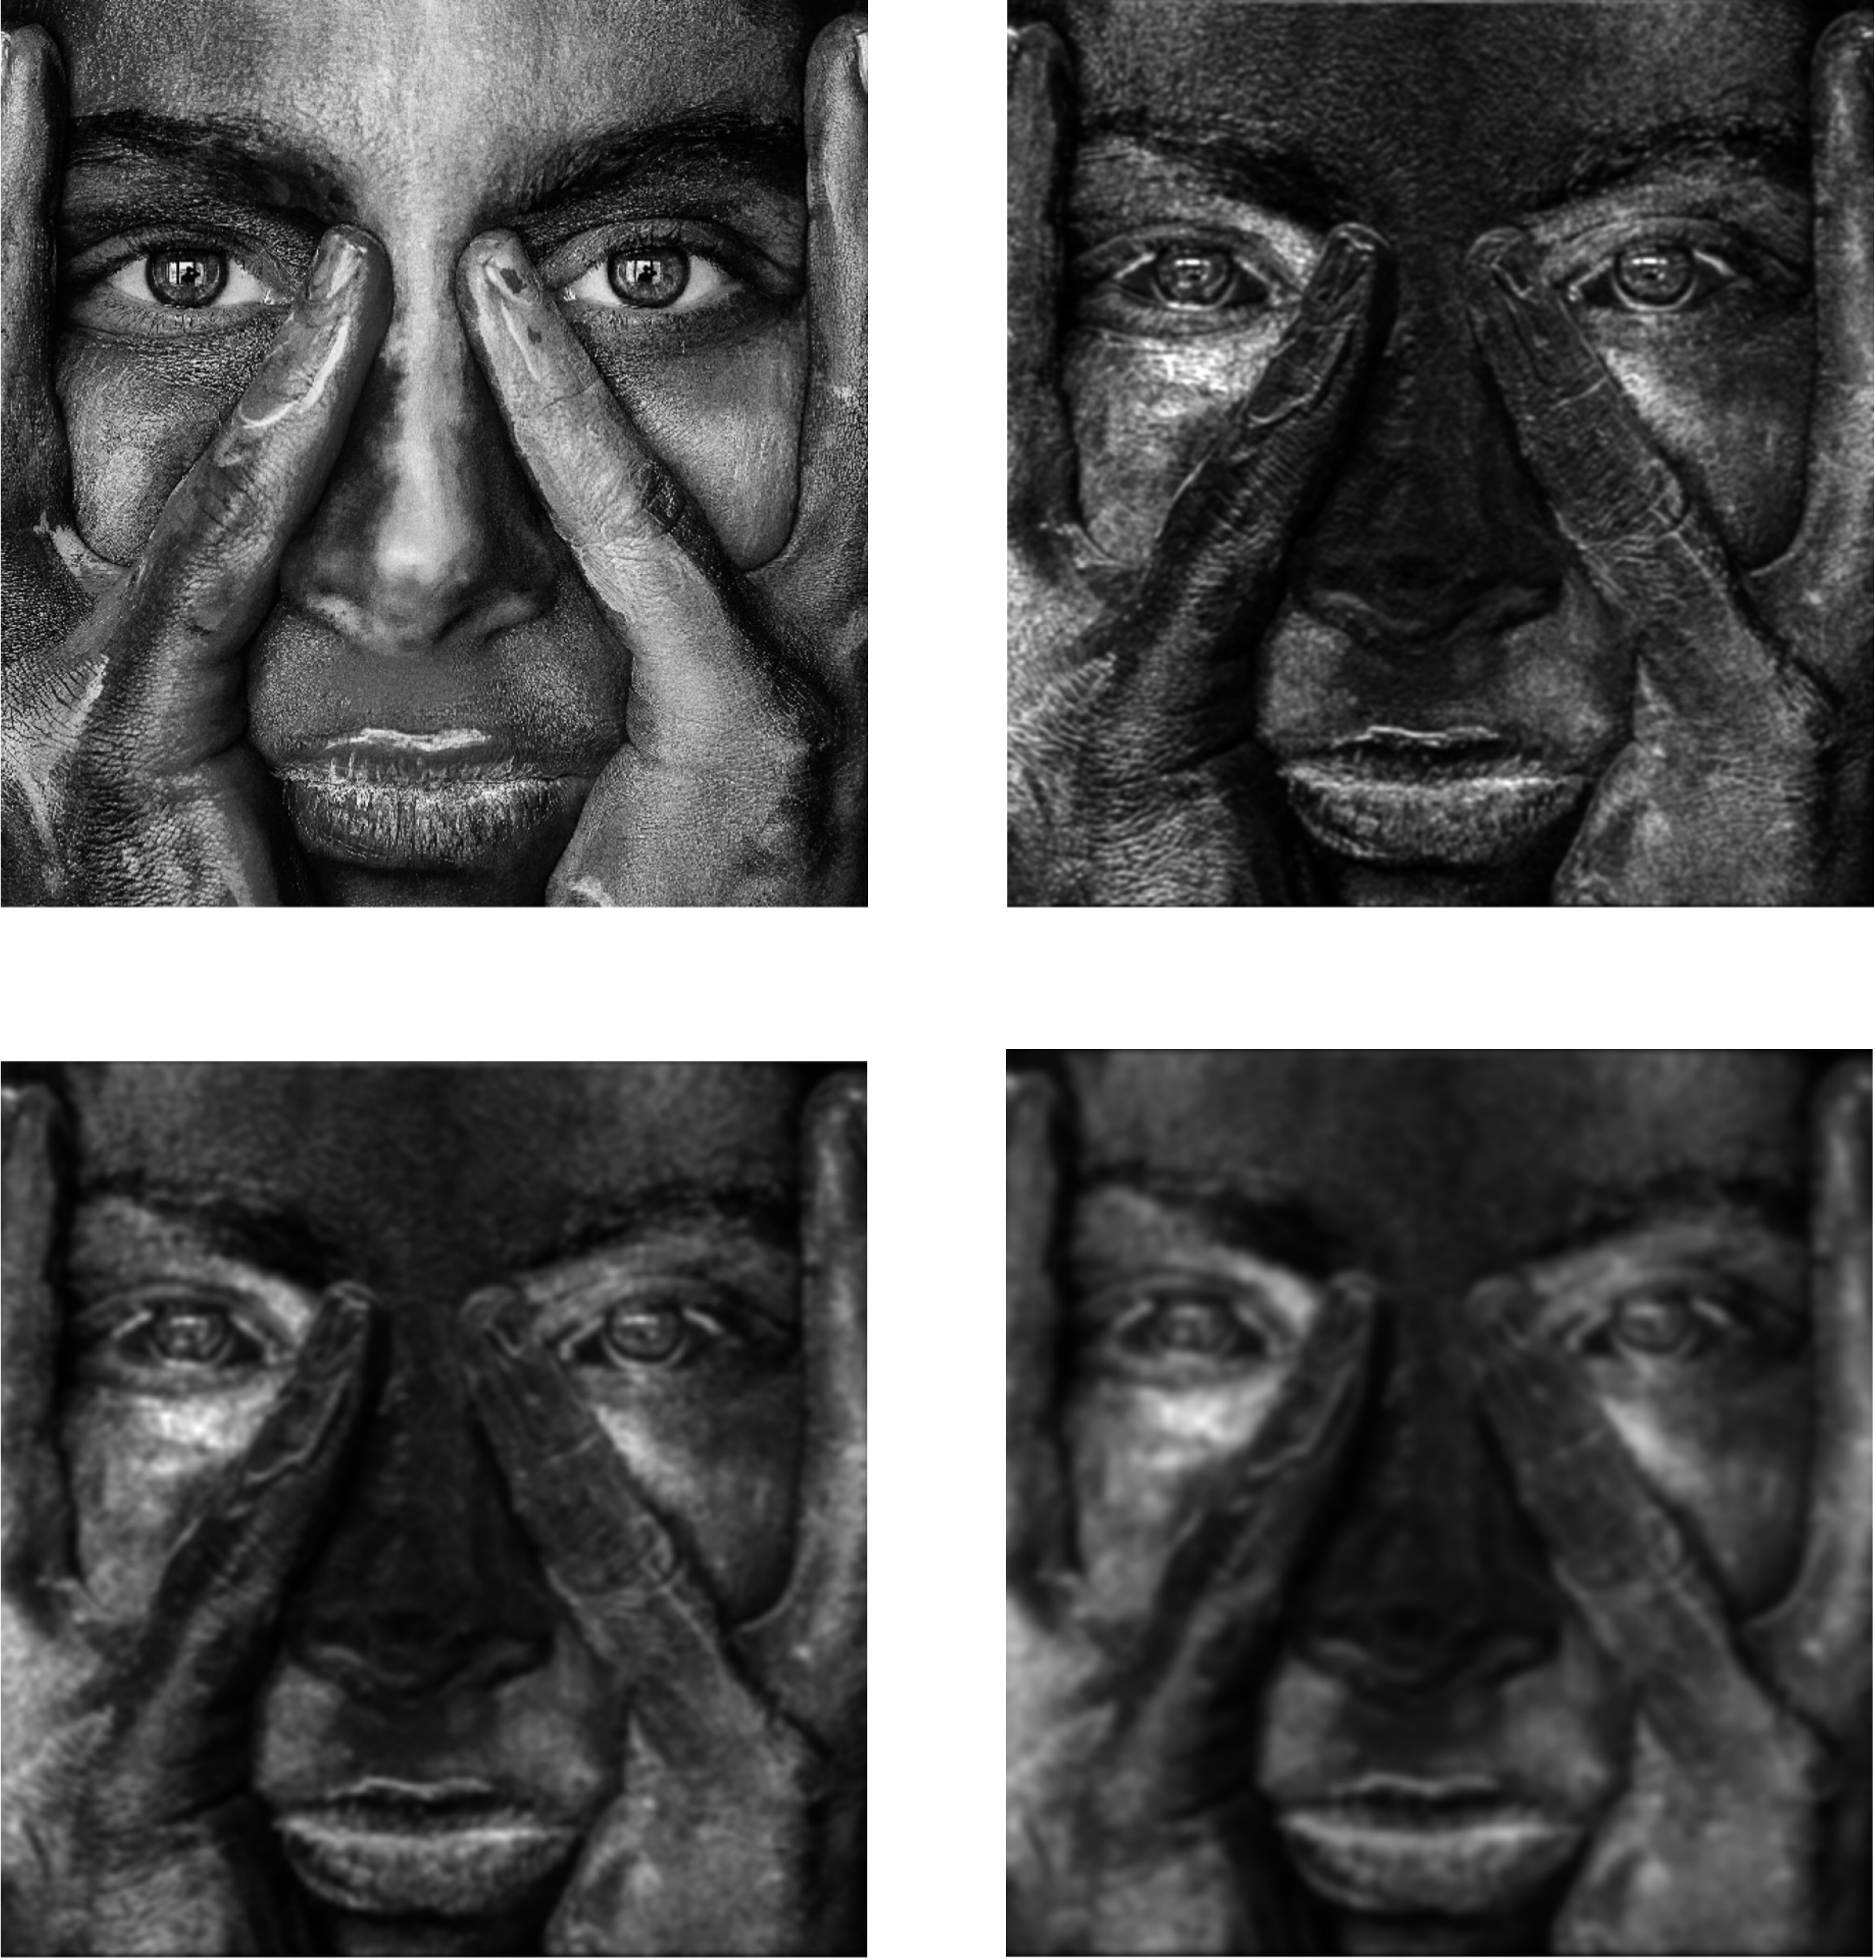
\includegraphics[width=\textwidth]{image1-table}
%   \caption{Three directional derivative images and the original in the top-left
%   corner}
% \end{figure}

\begin{figure}[h]\label{fig:grasshopper}
  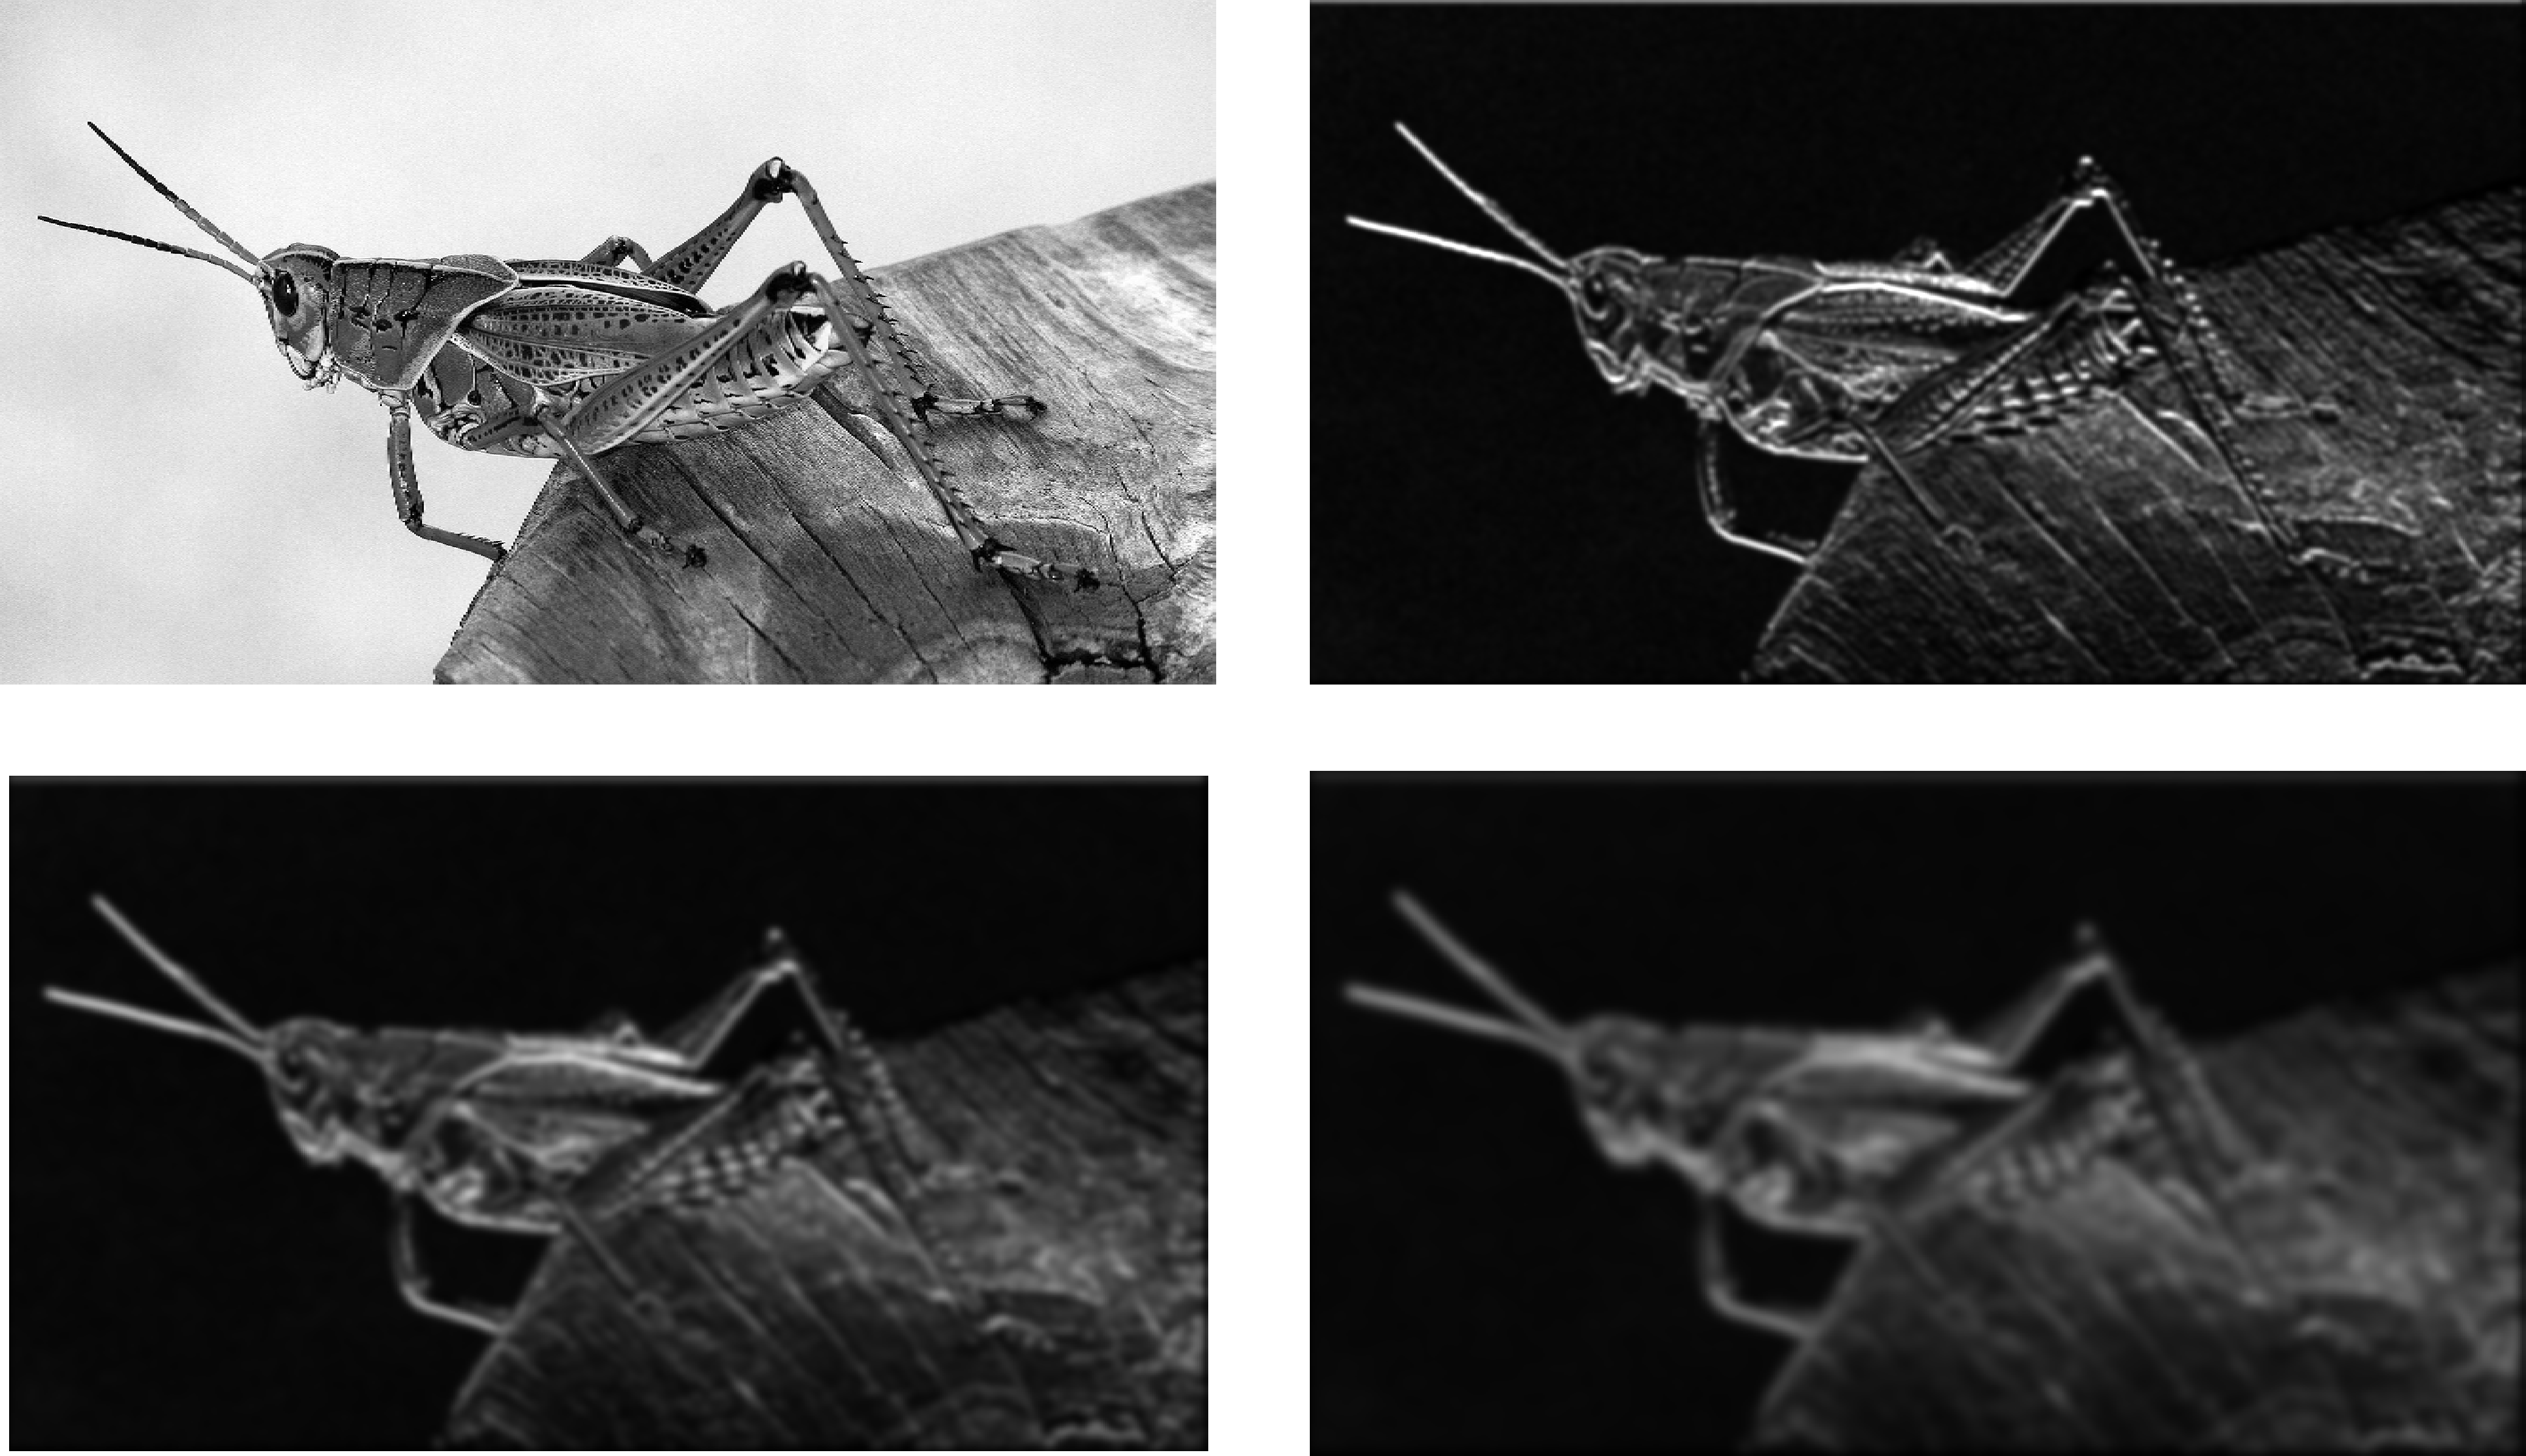
\includegraphics[width=\textwidth]{image2-table}
  \caption{Three directional derivative images and the original in the top-left
  corner.}
\end{figure}

\section{Description of feature points}

The Matlab DAISY code produces a descriptor for every pixel in the image. The
matrix's form is dictated by the given parameters. The rows of the matrix are
histograms. The number of histograms is \textbf{1 + the number of layers * the
number of histograms on each layer}. The columns in the matrix are the bins of
the histograms. The number of bins can also be controlled.

With the default parameters, the descriptor matrix for one pixel is of form
25$\times$8; 8 bins, 1 + 3 layers * 8 histograms per layer.
Figure~\ref{fig:histogram} shows one histogram of a descriptor for the pixel
(200, 200) from the figure~\ref{fig:grasshopper}.

\begin{figure}\label{fig:histogram}
  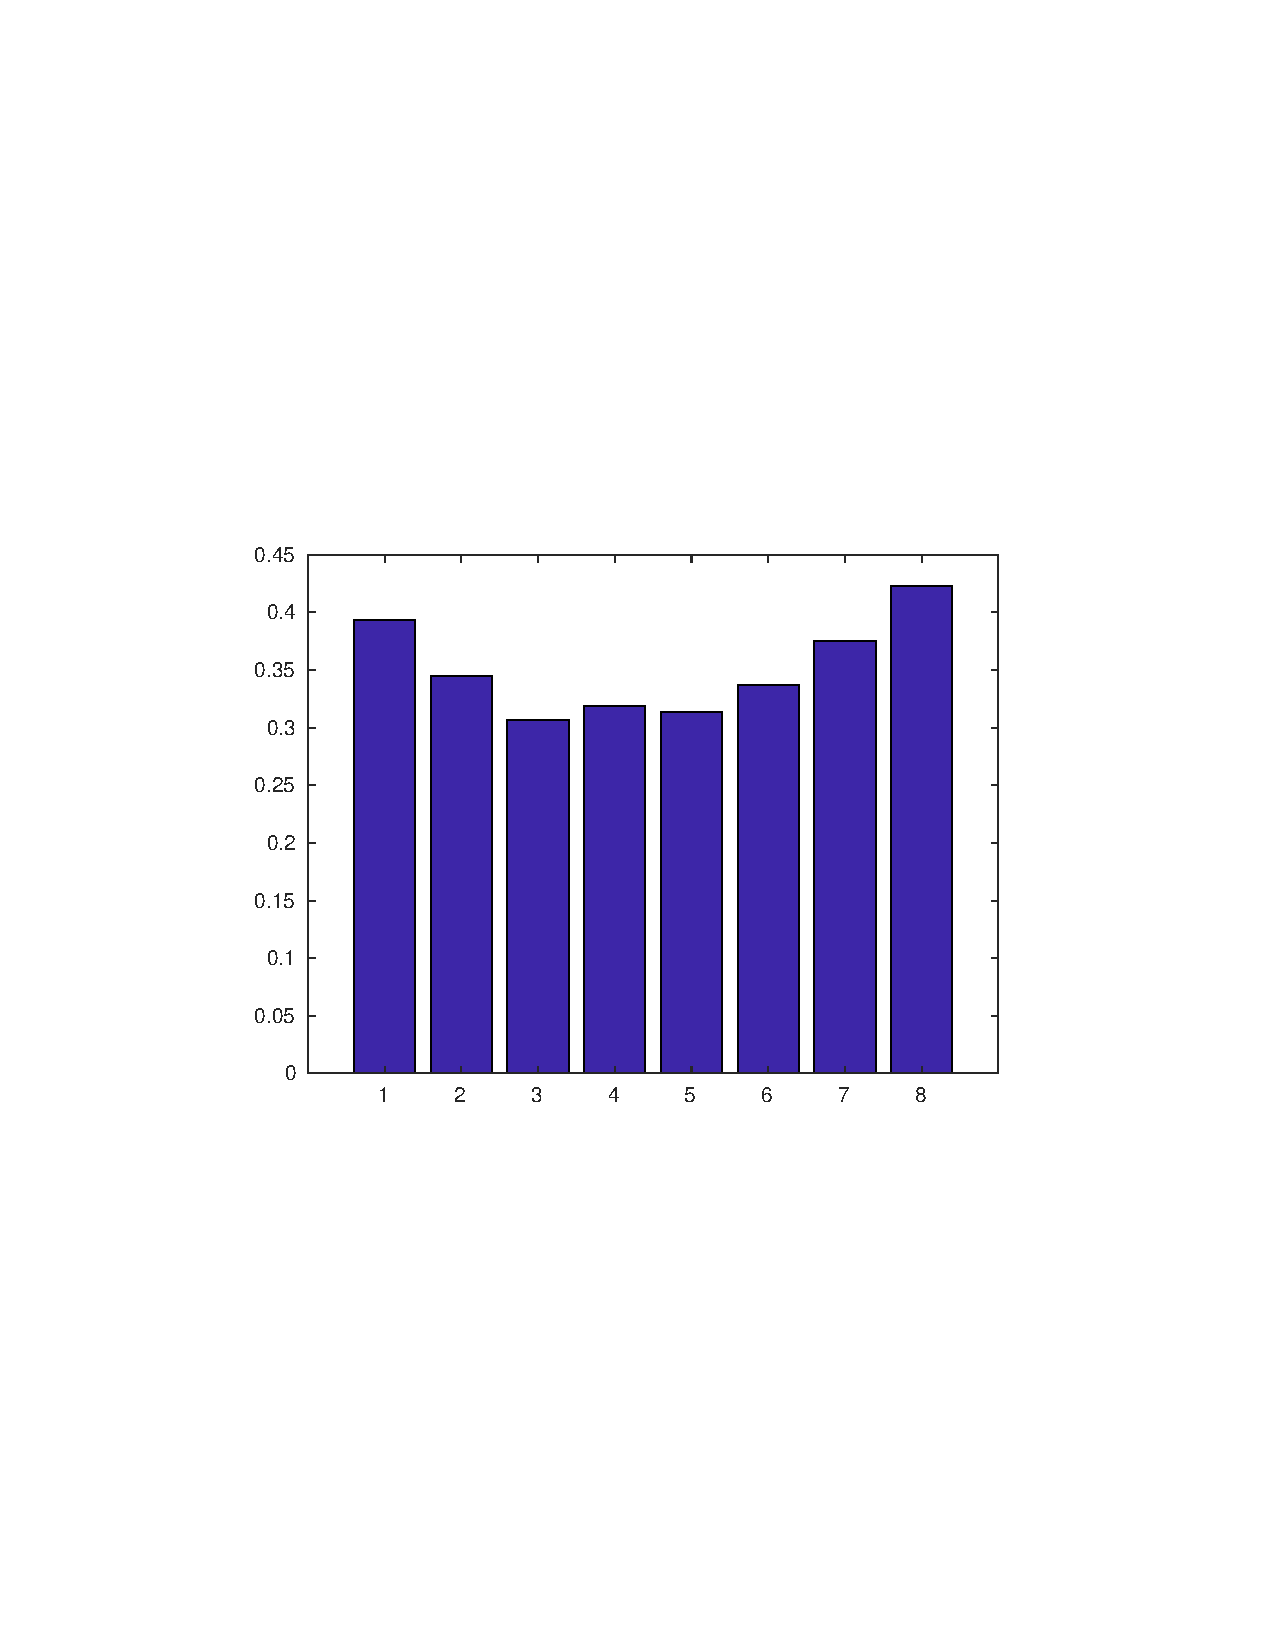
\includegraphics[width=\textwidth]{histogram}
  \caption{A row, ie.\ a histogram of a DAISY descriptor.}
\end{figure}

